% Options for packages loaded elsewhere
\PassOptionsToPackage{unicode}{hyperref}
\PassOptionsToPackage{hyphens}{url}
%
\documentclass[
]{article}
\usepackage{amsmath,amssymb}
\usepackage{lmodern}
\usepackage{iftex}
\ifPDFTeX
  \usepackage[T1]{fontenc}
  \usepackage[utf8]{inputenc}
  \usepackage{textcomp} % provide euro and other symbols
\else % if luatex or xetex
  \usepackage{unicode-math}
  \defaultfontfeatures{Scale=MatchLowercase}
  \defaultfontfeatures[\rmfamily]{Ligatures=TeX,Scale=1}
\fi
% Use upquote if available, for straight quotes in verbatim environments
\IfFileExists{upquote.sty}{\usepackage{upquote}}{}
\IfFileExists{microtype.sty}{% use microtype if available
  \usepackage[]{microtype}
  \UseMicrotypeSet[protrusion]{basicmath} % disable protrusion for tt fonts
}{}
\makeatletter
\@ifundefined{KOMAClassName}{% if non-KOMA class
  \IfFileExists{parskip.sty}{%
    \usepackage{parskip}
  }{% else
    \setlength{\parindent}{0pt}
    \setlength{\parskip}{6pt plus 2pt minus 1pt}}
}{% if KOMA class
  \KOMAoptions{parskip=half}}
\makeatother
\usepackage{xcolor}
\usepackage[margin=1in]{geometry}
\usepackage{graphicx}
\makeatletter
\def\maxwidth{\ifdim\Gin@nat@width>\linewidth\linewidth\else\Gin@nat@width\fi}
\def\maxheight{\ifdim\Gin@nat@height>\textheight\textheight\else\Gin@nat@height\fi}
\makeatother
% Scale images if necessary, so that they will not overflow the page
% margins by default, and it is still possible to overwrite the defaults
% using explicit options in \includegraphics[width, height, ...]{}
\setkeys{Gin}{width=\maxwidth,height=\maxheight,keepaspectratio}
% Set default figure placement to htbp
\makeatletter
\def\fps@figure{htbp}
\makeatother
\setlength{\emergencystretch}{3em} % prevent overfull lines
\providecommand{\tightlist}{%
  \setlength{\itemsep}{0pt}\setlength{\parskip}{0pt}}
\setcounter{secnumdepth}{-\maxdimen} % remove section numbering
\usepackage{helvet} \renewcommand\familydefault{\sfdefault}
\usepackage{booktabs}
\usepackage{longtable}
\usepackage{array}
\usepackage{multirow}
\usepackage{wrapfig}
\usepackage{float}
\usepackage{colortbl}
\usepackage{pdflscape}
\usepackage{tabu}
\usepackage{threeparttable}
\usepackage{threeparttablex}
\usepackage[normalem]{ulem}
\usepackage{makecell}
\usepackage{xcolor}
\ifLuaTeX
  \usepackage{selnolig}  % disable illegal ligatures
\fi
\IfFileExists{bookmark.sty}{\usepackage{bookmark}}{\usepackage{hyperref}}
\IfFileExists{xurl.sty}{\usepackage{xurl}}{} % add URL line breaks if available
\urlstyle{same} % disable monospaced font for URLs
\hypersetup{
  pdftitle={Lista 2 modulo 3},
  pdfauthor={César A. Galvão - 19/0011572},
  hidelinks,
  pdfcreator={LaTeX via pandoc}}

\title{Lista 2 modulo 3}
\author{César A. Galvão - 19/0011572}
\date{2022-09-20}

\begin{document}
\maketitle

\newpage{}

{
\setcounter{tocdepth}{3}
\tableofcontents
}
\let\oldsection\section
\renewcommand\section{\clearpage\oldsection}

\hypertarget{section}{%
\section*{}\label{section}}
\addcontentsline{toc}{section}{}

\hypertarget{efeitos-dos-fatores}{%
\subsection{Efeitos dos fatores}\label{efeitos-dos-fatores}}

Para calcular os efeitos dos fatores, calcula-se os totais (\(a\),
\(b\), \(ab\) e \((1)\)) utilizando os seguintes contrastes:

\begin{longtable}{cccc}
\toprule
Totais & A & B & AB\\
\midrule
\endfirsthead
\multicolumn{4}{@{}l}{\textit{(continued)}}\\
\toprule
Totais & A & B & AB\\
\midrule
\endhead

\endfoot
\bottomrule
\endlastfoot
\cellcolor{gray!15}{(1)} & \cellcolor{gray!15}{-1} & \cellcolor{gray!15}{-1} & \cellcolor{gray!15}{1}\\
a & 1 & -1 & -1\\
\cellcolor{gray!15}{b} & \cellcolor{gray!15}{-1} & \cellcolor{gray!15}{1} & \cellcolor{gray!15}{-1}\\
ab & 1 & 1 & 1\\*
\end{longtable}

Para calcular a magnitude do efeito A, por exemplo, calcula-se:

\begin{align}
  A = \frac{a+ab-b-(1)}{2n} = \frac{58.081 + 59.299 + 55.686 + 59.156}{8} = -0.31725
\end{align}

Obtem-se dessa forma os seguintes efeitos:

\begin{longtable}{ccc}
\toprule
A & B & AB\\
\midrule
\endfirsthead
\multicolumn{3}{@{}l}{\textit{(continued)}}\\
\toprule
A & B & AB\\
\midrule
\endhead

\endfoot
\bottomrule
\endlastfoot
\cellcolor{gray!15}{-0.3173} & \cellcolor{gray!15}{0.586} & \cellcolor{gray!15}{0.2815}\\*
\end{longtable}

\hypertarget{anuxe1lise-de-variuxe2ncia}{%
\subsection{Análise de variância}\label{anuxe1lise-de-variuxe2ncia}}

É possível observar na tabela de ANOVA a seguir que as diferenças entre
níveis dos fatores não são significativas com \(\alpha = 0,05\), bem
como a interação entre os fatores.

\begin{longtable}{lccccl}
\toprule
Fonte de variação & g.l. & SQ & MQ & Estatística F & p-valor\\
\midrule
\endfirsthead
\multicolumn{6}{@{}l}{\textit{(continued)}}\\
\toprule
Fonte de variação & g.l. & SQ & MQ & Estatística F & p-valor\\
\midrule
\endhead

\endfoot
\bottomrule
\endlastfoot
\cellcolor{gray!15}{A} & \cellcolor{gray!15}{1} & \cellcolor{gray!15}{0.4026} & \cellcolor{gray!15}{0.4026} & \cellcolor{gray!15}{1.2619} & \cellcolor{gray!15}{0.2833}\\
B & 1 & 1.3736 & 1.3736 & 4.3054 & 0.0602\\
\cellcolor{gray!15}{A:B} & \cellcolor{gray!15}{1} & \cellcolor{gray!15}{0.3170} & \cellcolor{gray!15}{0.3170} & \cellcolor{gray!15}{0.9935} & \cellcolor{gray!15}{0.3386}\\
Residuals & 12 & 3.8285 & 0.3190 & NA & NA\\*
\end{longtable}

\hypertarget{modelo-de-efeitos-e-estimadores}{%
\subsection{Modelo de efeitos e
estimadores}\label{modelo-de-efeitos-e-estimadores}}

Considera-se o seguinte modelo de efeitos teórico

\begin{align}
  y_{ijk} = \mu + \tau_i + \beta_j + (\tau\beta)_{ij} + \varepsilon_{ijk}, \quad
  \begin{cases}
    i = 1, ..., a\\
    j = 1, ..., b\\
    k = 1, ..., n
  \end{cases}
\end{align}

em que \(\mu\) é média geral da variável resposta, \(\tau_i\) do i-ésimo
nível do tratamento A, \(\beta_j\) do j-ésimo nível do tratamento B,
\((\tau\beta)_{ij}\) é o efeito da interação dos fatores A e B e
\(\varepsilon_{ijk}\) é o erro aleatório.

Considera-se como hipóteses nulas para a análise de variância a
igualdade entre os níveis de cada tratamento e como hipóteses
alternativas a existência de pelo menos um nível diferente dos demais.

Conforme a tabela de análise de variância apresentada, não foram
rejeitadas as hipóteses nulas para nenhum dos tratamentos e, portanto,
poderíamos considerar o modelo reduzido

\begin{align}
  y_{ijk} = \mu + \varepsilon_{ijk}, \quad
  \begin{cases}
    i = 1, ..., a\\
    j = 1, ..., b\\
    k = 1, ..., n
  \end{cases}
\end{align}

em que a variância pode ser explicada unicamente pelo erro aleatório.

Para efeito de exercício, calculamos os estimadores:

\begin{longtable}{cc}
\toprule
$\hat{\mu}$ & $\hat{\sigma}^2$\\
\midrule
\endfirsthead
\multicolumn{2}{@{}l}{\textit{(continued)}}\\
\toprule
$\hat{\mu}$ & $\hat{\sigma}^2$\\
\midrule
\endhead

\endfoot
\bottomrule
\endlastfoot
\cellcolor{gray!15}{14.51} & \cellcolor{gray!15}{0.32}\\*
\end{longtable}

\begin{longtable}{cccccc}
\toprule
$\tau_1$ & $\tau_2$ & $\beta_1$ & $\beta_2$ & $(\tau\beta)_1$ & $(\tau\beta)_2$\\
\midrule
\endfirsthead
\multicolumn{6}{@{}l}{\textit{(continued)}}\\
\toprule
$\tau_1$ & $\tau_2$ & $\beta_1$ & $\beta_2$ & $(\tau\beta)_1$ & $(\tau\beta)_2$\\
\midrule
\endhead

\endfoot
\bottomrule
\endlastfoot
\cellcolor{gray!15}{0.159} & \cellcolor{gray!15}{-0.159} & \cellcolor{gray!15}{-0.293} & \cellcolor{gray!15}{0.293} & \cellcolor{gray!15}{-0.141} & \cellcolor{gray!15}{0.141}\\*
\end{longtable}

\hypertarget{gruxe1fico-de-interauxe7uxe3o}{%
\subsection{Gráfico de interação}\label{gruxe1fico-de-interauxe7uxe3o}}

O gráfico de interação a seguir sugere uma diferença entre níveis de
resposta para o fator A quando o fator B está em nível baixo, mas não
sugerem o mesmo para o nível alto do fator B. Além disso, o nível de
resposta parece aumentar genericamente quando se aumenta o nível do
fator B.

\begin{center}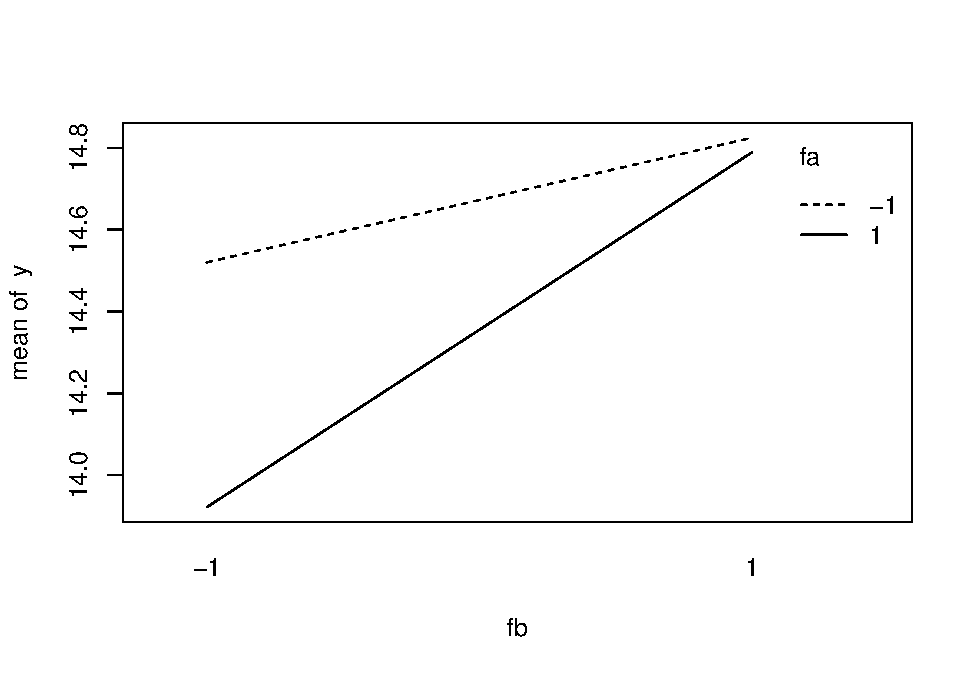
\includegraphics[width=0.6\linewidth]{lista9_files/figure-latex/graf-interacao-1} \end{center}

Já o seguinte sugere haver uma diferença maior entre os níveis de
resposta quando se aumenta o fator A. O desempenho com nível baixo do
fator B já parece inferior com nível baixo de A e parece decrescer
quando se aumenta o nível de A. Já o nível alto de B parece pouco
afetado em relação à variação de A.

\begin{center}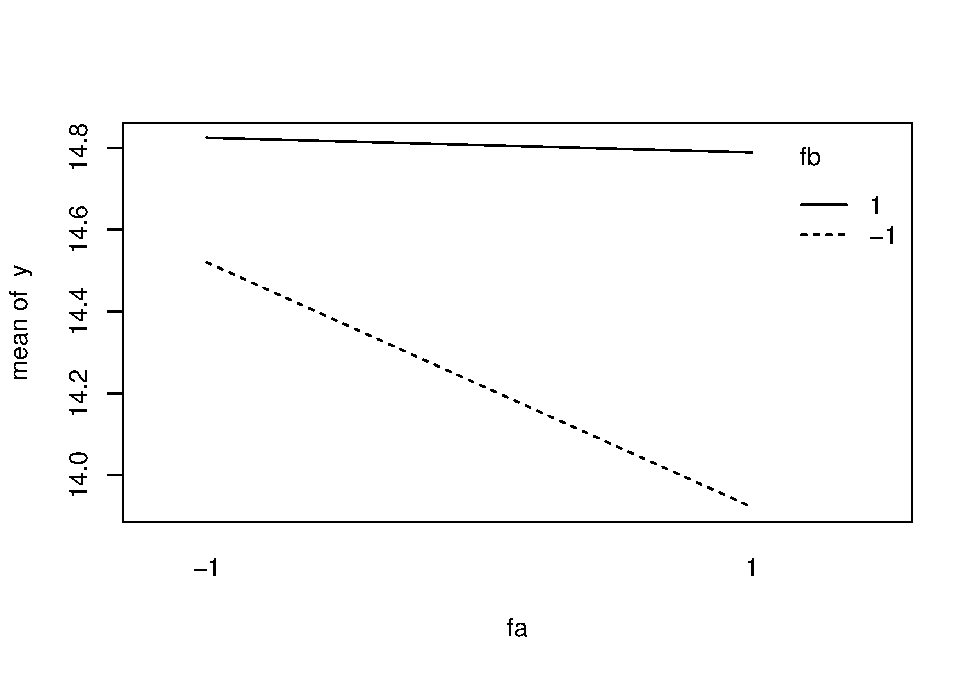
\includegraphics[width=0.6\linewidth]{lista9_files/figure-latex/graf-interacao2-1} \end{center}

\hypertarget{modelo-de-regressuxe3o-linear}{%
\subsection{Modelo de regressão
linear}\label{modelo-de-regressuxe3o-linear}}

Considerando as variáveis codificadas \(X_1, X_2 \in \{-1, 1\}\)
correspondentes a níveis baixos e altos dos fatores A, B e a interação
AB (\(X_1X_2\)), é possível construir um modelo de regressão linear.
Seus coeficientes estimados por mínimos quadrados ordinários são obtidos
como a metade da magnitude de efeito dos fatores e o intercepto é obtido
pela média geral da amostra.

\begin{align}
  \hat{y} &= \hat{\beta}_0 + \hat{\beta}_1 X_1 + \hat{\beta}_2 X2 + \hat{\beta}_3 X_1X_2 \nonumber \\
   &= 14.514 - 0.152 X_1 + 0.293 X_2 +  0.14 X_1X_2 \label{modelo_lin}
\end{align}

\hypertarget{gruxe1fico-de-superfuxedcie}{%
\subsection{Gráfico de superfície}\label{gruxe1fico-de-superfuxedcie}}

O gráfico de superfície correspondente a (\ref{modelo_lin}) é exibido a
seguir:

\begin{center}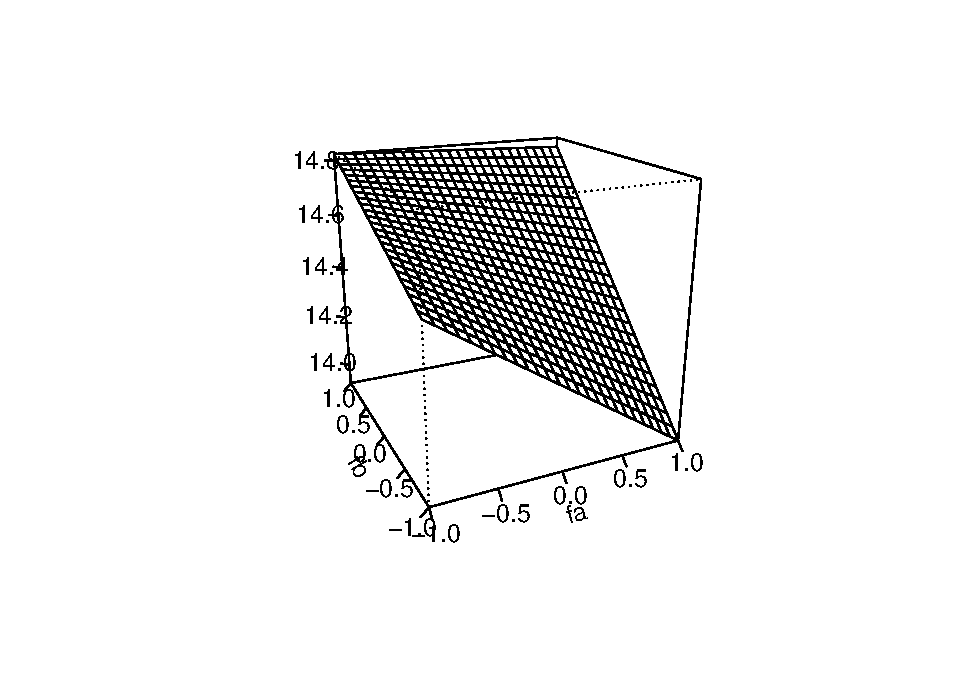
\includegraphics[width=0.75\linewidth]{lista9_files/figure-latex/superficie-1} \end{center}

\hypertarget{projeuxe7uxe3o-de-resposta}{%
\subsection{Projeção de resposta}\label{projeuxe7uxe3o-de-resposta}}

Para facilitar a análise e identicar níveis de resposta, podemos também
avaliar graficamente os níveis de resposta utilizando o gráfico de
curvas de nível a seguir.

\begin{center}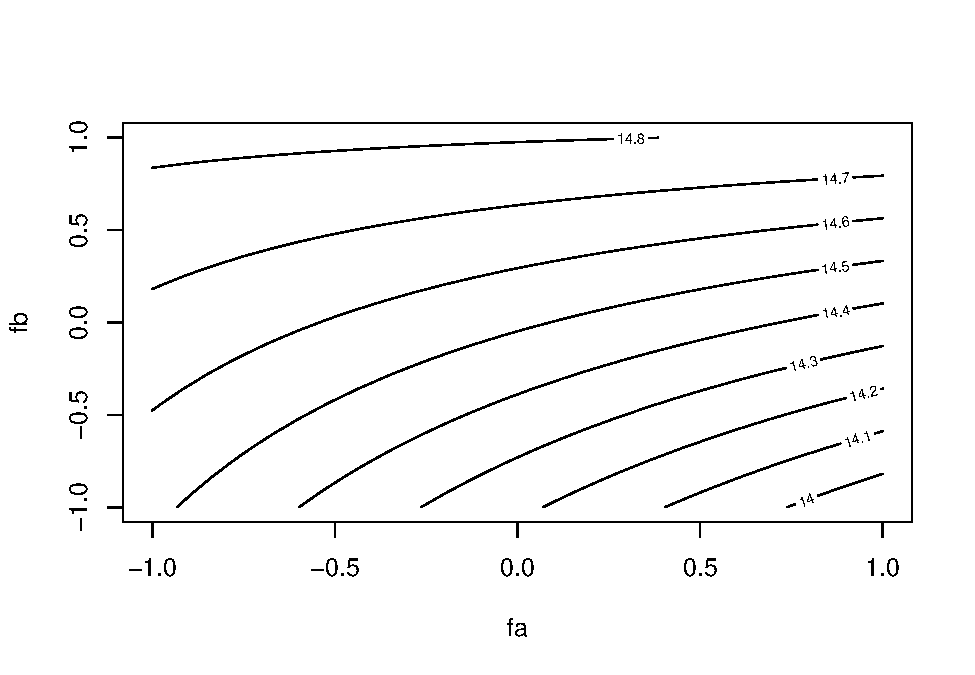
\includegraphics[width=0.75\linewidth]{lista9_files/figure-latex/curvas-nivel-1} \end{center}

Se desejamos obter um valor de 14.5\(\mu m\) na variável resposta,
podemos inicialmente tentar seguir a curva de nível correspondente no
gráfico de curvas. Enquanto não fica claro qual deveria ser o nível do
fator B se utilizamos o fator A em nível alto, o gráfico evidencia que
ambos os fatores em nível baixo deveriam render a resposta desejada.

Para auxiliar a análise, construimos intervalos de confiança com
\(\alpha = 0,95\) para a média de cada ponto fatorial. Como já avaliado,
o ponto em que ambos os fatores têm nível baixo tem a média centrada
exatamente no nível de resposta desejado, enquanto outros dois pontos
teriam a média um pouco deslocada porém com IC que conteriam o valor
desejado. Conclui-se que a recomendação seria a opção de fatores A e B
ambos em nível baixo.

\begin{longtable}{ccccc}
\toprule
A & B & LI & $\bar{Y}$ & LS\\
\midrule
\endfirsthead
\multicolumn{5}{@{}l}{\textit{(continued)}}\\
\toprule
A & B & LI & $\bar{Y}$ & LS\\
\midrule
\endhead

\endfoot
\bottomrule
\endlastfoot
\cellcolor{gray!15}{-1} & \cellcolor{gray!15}{-1} & \cellcolor{gray!15}{14.013} & \cellcolor{gray!15}{14.520} & \cellcolor{gray!15}{15.028}\\
1 & -1 & 13.414 & 13.922 & 14.429\\
\cellcolor{gray!15}{-1} & \cellcolor{gray!15}{1} & \cellcolor{gray!15}{14.317} & \cellcolor{gray!15}{14.825} & \cellcolor{gray!15}{15.332}\\
1 & 1 & 14.281 & 14.789 & 15.297\\*
\end{longtable}

\end{document}
